\documentclass[letterpaper,10pt]{article}
\usepackage{mathpazo}
\usepackage{authblk}
\usepackage{amsmath}
\usepackage{subcaption}

\usepackage{tikz}
\usetikzlibrary{arrows,patterns}

\usepackage{color}
\definecolor{green}{HTML}{859900}
\definecolor{darkblue}{HTML}{3399cc}
\definecolor{darkred}{HTML}{993333}

\usepackage[colorlinks=true,linkcolor=blue,citecolor=red]{hyperref}

\begin{document}

\title{Normalizing $\boldsymbol{\chi}(-2\omega;\omega,\omega)$ for Specific
Cases}
\author[1]{Sean M. Anderson}
\author[1]{Bernardo S. Mendoza}
\affil[1]{Centro de Investigaciones en \'Optica, A.C., Le\'on 37150, Mexico}

\maketitle

%%%%%%%%%%%%%%%%%%%%%%%%%%%%%%%%%%%%%%%%%%%%%%%%%%%%%%%%%%%%%%%%%%%%%%%%%%%%%%%%
%%%%%%%%%%%%%%%%%%%%%%%%%%%%%%%%%%%%%%%%%%%%%%%%%%%%%%%%%%%%%%%%%%%%%%%%%%%%%%%%

\section*{First Case: Bulk Materials}

Let us first consider the case of a bulk material, that is conformed entirely of
a supercell with no vacuum region. A unit cell is repeated indefinitely in every
direction, thus creating a three-dimensional reproduction of an infinite
material. From Fig. \ref{fig:bulk}, we can see that the volume of each unit cell
is $\Omega = L^{3}$. We calculate $\boldsymbol{\chi}(-2\omega;\omega,\omega)$
using the TINIBA \cite{tiniba} software suite; for ease of notation,
$\boldsymbol{\chi}(-2\omega;\omega,\omega) = \boldsymbol{\chi}_{T}$ ($T$ for
TINIBA).

\begin{figure}[b]
\centering
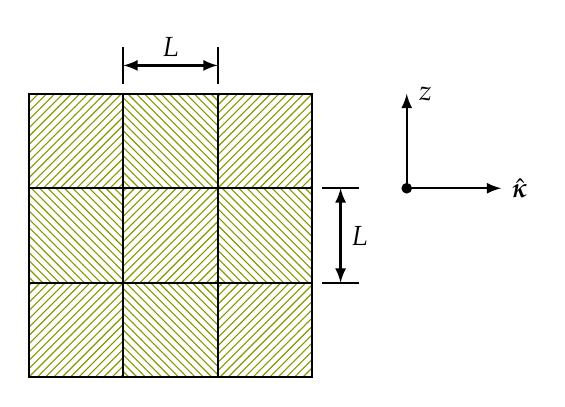
\begin{tikzpicture}[scale=1.2]
% axes
\draw [latex-latex,thick] (4,3) -- (4,2) -- (5,2);
\draw [fill=black] (4,2) circle (0.05);
\node at (4.2,3) {$z$};
\node at (5.2,2) {$\hat{\boldsymbol{\kappa}}$};
% hatched squares
\draw[thick,pattern=north east lines,pattern color=green] (0,0) rectangle (1,1);
\draw[thick,pattern=north west lines,pattern color=green] (0,1) rectangle (1,2);
\draw[thick,pattern=north east lines,pattern color=green] (0,2) rectangle (1,3);
\draw[thick,pattern=north west lines,pattern color=green] (1,0) rectangle (2,1);
\draw[thick,pattern=north east lines,pattern color=green] (1,1) rectangle (2,2);
\draw[thick,pattern=north west lines,pattern color=green] (1,2) rectangle (2,3);
\draw[thick,pattern=north east lines,pattern color=green] (2,0) rectangle (3,1);
\draw[thick,pattern=north west lines,pattern color=green] (2,1) rectangle (3,2);
\draw[thick,pattern=north east lines,pattern color=green] (2,2) rectangle (3,3);
% right label
\draw[thick] (3.1,1) to (3.5,1);
\draw[thick] (3.1,2) to (3.5,2);
\draw[thick,latex-latex] (3.3,1) to (3.3,2);
\node at (3.5,1.5) {$L$};
% top label
\draw[thick] (1,3.1) to (1,3.5);
\draw[thick] (2,3.1) to (2,3.5);
\draw[thick,latex-latex] (1,3.3) to (2,3.3);
\node at (1.5,3.5) {$L$};
\end{tikzpicture}
\caption{The bulk supercell is repeated indefinitely along the $z$ and
$\hat{\boldsymbol{\kappa}}$ axes. There is only material present, with no vacuum
region between each repeat.}
\label{fig:bulk}
\end{figure}

For the bulk calculation, $\boldsymbol{\chi}_{T}$ must be normalized over the
volume of the unit cell (i.e. $1/\Omega$); this normalization happens
automatically in TINIBA. Thus, no further action is necessary and the
susceptibility can be used as is. Finally, we establish that
$\boldsymbol{\chi}_{T} = \boldsymbol{\chi}_{b}$, where $\boldsymbol{\chi}_{b}$
is the desired susceptibility for our bulk system. Calculated in this fashion,
$\boldsymbol{\chi}_{b}$ has the appropriate MKS units of m/V.


%%%%%%%%%%%%%%%%%%%%%%%%%%%%%%%%%%%%%%%%%%%%%%%%%%%%%%%%%%%%%%%%%%%%%%%%%%%%%%%%
%%%%%%%%%%%%%%%%%%%%%%%%%%%%%%%%%%%%%%%%%%%%%%%%%%%%%%%%%%%%%%%%%%%%%%%%%%%%%%%%

\section*{Second Case: Surfaces}

Now, we will consider calculating $\boldsymbol{\chi}(-2\omega;\omega,\omega)$
for surfaces. This is done following the theoretical framework established in
Ref. \cite{andersonPRB15}. Just as for the bulk case, we use the supercell
method that repeats each cell across all directions (see Fig.
\ref{fig:surface}). However, we represent the surface by using a slab of
material with finite height; this necessarily implies that there are regions of
empty space between each repeat. The slab has both upper and lower surfaces, and
we can extract the response for each by use of the cut function.

\begin{figure}[h]
\centering
\subcaptionbox{Repeated supercells for a surface material. Each individual
supercell is repeated in every direction, just like the bulk case. Vacuum
regions must be included, seperating each
supercell.\label{fig:sf_repeat}}[0.45\linewidth]
{
\centering
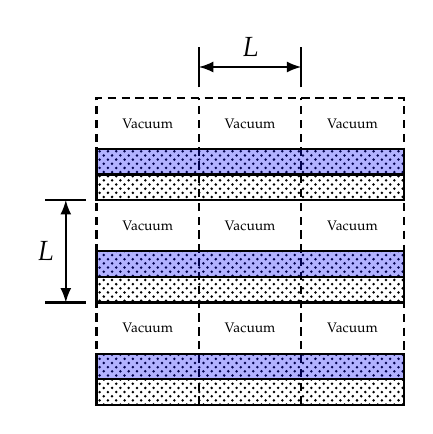
\begin{tikzpicture}[scale=1.3]
% outside dashed lines
\draw[thick,densely dashed] (0.5,0) rectangle (3.5,3);
% vertical dashed line
\draw[thick,densely dashed] (1.5,0) to (1.5,3);
\draw[thick,densely dashed] (2.5,0) to (2.5,3);
% entire slab
\draw[thick,pattern=crosshatch dots] (0.5,0) rectangle (3.5,0.5);
\draw[thick,pattern=crosshatch dots] (0.5,1) rectangle (3.5,1.5);
\draw[thick,pattern=crosshatch dots] (0.5,2) rectangle (3.5,2.5);
% half slab
\draw[thick,fill=blue,fill opacity=0.3] (0.5,0.25) rectangle (3.5,0.5);
\draw[thick,fill=blue,fill opacity=0.3] (0.5,1.25) rectangle (3.5,1.5);
\draw[thick,fill=blue,fill opacity=0.3] (0.5,2.25) rectangle (3.5,2.5);
% vacuum labels
\node at (1,0.75) {\tiny Vacuum};
\node at (2,0.75) {\tiny Vacuum};
\node at (3,0.75) {\tiny Vacuum};
\node at (1,1.75) {\tiny Vacuum};
\node at (2,1.75) {\tiny Vacuum};
\node at (3,1.75) {\tiny Vacuum};
\node at (1,2.75) {\tiny Vacuum};
\node at (2,2.75) {\tiny Vacuum};
\node at (3,2.75) {\tiny Vacuum};
% left label
\draw[thick] (0,1) to (0.4,1);
\draw[thick] (0,2) to (0.4,2);
\draw[thick,latex-latex] (0.2,1) to (0.2,2);
\node at (0,1.5) {$L$};
% top label
\draw[thick] (1.5,3.1) to (1.5,3.5);
\draw[thick] (2.5,3.1) to (2.5,3.5);
\draw[thick,latex-latex] (1.5,3.3) to (2.5,3.3);
\node at (2,3.5) {$L$};
\end{tikzpicture}
}
\hfill
\subcaptionbox{An individual supercell, which consists of a slab (with upper and
bottom surfaces) and a vacuum region. The total height will be the combined
height of the vacuum region and the slab
($L_{s}$).\label{fig:sf_supercell}}[0.45\linewidth]
{
\centering
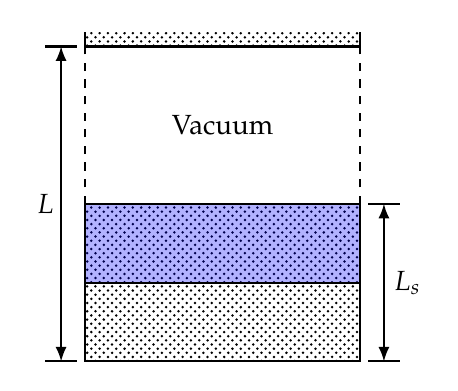
\begin{tikzpicture}
% outside lines
\draw[thick,dashed] (0.5,2) to (0.5,4);
\draw[thick,dashed] (4,2) to (4,4);
% rectangles
\draw[thick,pattern=crosshatch dots] (0.5,0) rectangle (4,2);
\draw[thick,fill=blue,fill opacity=0.3] (0.5,1) rectangle (4,2);
\draw[thick,pattern=crosshatch dots] (0.5,4) rectangle (4,4.2);
\draw[ultra thick,white] (0.4,4.21) to (4.1,4.21);
\node at (2.25,3) {Vacuum};
% right label
\draw[thick] (4.1,0) to (4.5,0);
\draw[thick] (4.1,2) to (4.5,2);
\draw[thick,latex-latex] (4.3,0) to (4.3,2);
\node at (4.6,1) {$L_{s}$};
% left label
\draw[thick] (0,0) to (0.4,0);
\draw[thick] (0,4) to (0.4,4);
\draw[thick,latex-latex] (0.2,0) to (0.2,4);
\node at (0,2) {$L$};
\end{tikzpicture}
}
\caption{Just like for the bulk case, we use the supercell scheme for
calculating $\boldsymbol{\chi}(-2\omega;\omega,\omega)$ for surfaces.}
\label{fig:surface}
\end{figure}

Fig. \ref{fig:sf_supercell} depicts a representative supercell for a surface material. As mentioned above, it is necessary to include the cut-function to extract the surface response. For instance, a centrosymmetric material will always yield $\boldsymbol{\chi}(-2\omega;\omega,\omega) = 0$, except at the surface where the symmetry is broken. If we calculate the response from the entire slab, the contribution from the bottom half will cancel out the top half; thus, we use the cut function to only calculate over the desired region. For most surfaces, we can simply 

The blue shaded region represents the \emph{half-slab}

%%%%%%%%%%%%%%%%%%%%%%%%%%%%%%%%%%%%%%%%%%%%%%%%%%%%%%%%%%%%%%%%%%%%%%%%%%%%%%%%
%%%%%%%%%%%%%%%%%%%%%%%%%%%%%%%%%%%%%%%%%%%%%%%%%%%%%%%%%%%%%%%%%%%%%%%%%%%%%%%%

\section*{Third Case: Two-dimensional Materials}

\begin{figure}[t]
\centering
\subcaptionbox{Repeated supercells for a 2D material. Again, each individual
supercell is repeated in every direction. Vacuum regions seperate each slab of
material.}[0.45\linewidth]
{
\centering
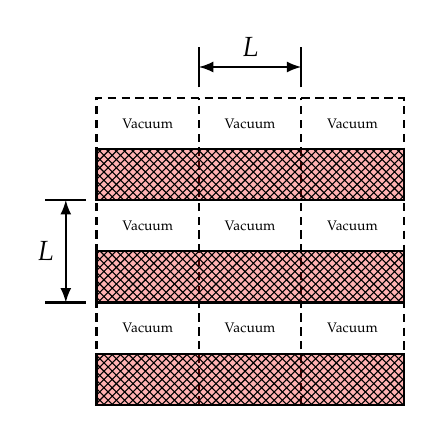
\begin{tikzpicture}[scale=1.3]
% outside dashed lines
\draw[thick,densely dashed] (0.5,0) rectangle (3.5,3);
% vertical dashed line
\draw[thick,densely dashed] (1.5,0) to (1.5,3);
\draw[thick,densely dashed] (2.5,0) to (2.5,3);
% entire slab
\draw[thick,pattern=crosshatch,preaction={fill=red,fill opacity=0.3}] (0.5,0) rectangle (3.5,0.5);
\draw[thick,pattern=crosshatch,preaction={fill=red,fill opacity=0.3}] (0.5,1) rectangle (3.5,1.5);
\draw[thick,pattern=crosshatch,preaction={fill=red,fill opacity=0.3}] (0.5,2) rectangle (3.5,2.5);
% vacuum labels
\node at (1,0.75) {\tiny Vacuum};
\node at (2,0.75) {\tiny Vacuum};
\node at (3,0.75) {\tiny Vacuum};
\node at (1,1.75) {\tiny Vacuum};
\node at (2,1.75) {\tiny Vacuum};
\node at (3,1.75) {\tiny Vacuum};
\node at (1,2.75) {\tiny Vacuum};
\node at (2,2.75) {\tiny Vacuum};
\node at (3,2.75) {\tiny Vacuum};
% left label
\draw[thick] (0,1) to (0.4,1);
\draw[thick] (0,2) to (0.4,2);
\draw[thick,latex-latex] (0.2,1) to (0.2,2);
\node at (0,1.5) {$L$};
% top label
\draw[thick] (1.5,3.1) to (1.5,3.5);
\draw[thick] (2.5,3.1) to (2.5,3.5);
\draw[thick,latex-latex] (1.5,3.3) to (2.5,3.3);
\node at (2,3.5) {$L$};
\end{tikzpicture}
\label{fig:2d_repeat}
}
\hfill
\subcaptionbox{An individual supercell, with slab and vacuum region. We
calculate the response from the entire slab, disregarding any
layers.}[0.45\linewidth]
{
\centering
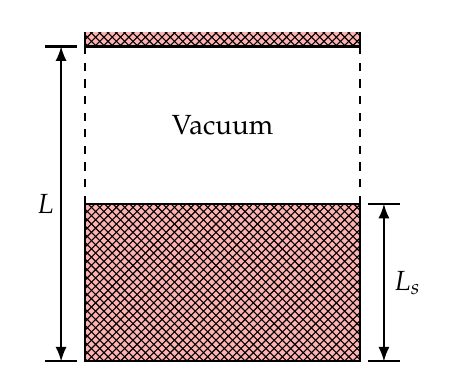
\begin{tikzpicture}
% outside lines
\draw[thick,dashed] (0.5,2) to (0.5,4);
\draw[thick,dashed] (4,2) to (4,4);
% rectangles
\draw[thick,pattern=crosshatch,preaction={fill=red,fill opacity=0.3}] (0.5,0) rectangle (4,2);
\draw[thick,pattern=crosshatch,preaction={fill=red,fill opacity=0.3}] (0.5,4) rectangle (4,4.2);
\draw[ultra thick,white] (0.4,4.21) to (4.1,4.21);
\node at (2.25,3) {Vacuum};
% right label
\draw[thick] (4.1,0) to (4.5,0);
\draw[thick] (4.1,2) to (4.5,2);
\draw[thick,latex-latex] (4.3,0) to (4.3,2);
\node at (4.6,1) {$L_{s}$};
% left label
\draw[thick] (0,0) to (0.4,0);
\draw[thick] (0,4) to (0.4,4);
\draw[thick,latex-latex] (0.2,0) to (0.2,4);
\node at (0,2) {$L$};
\end{tikzpicture}
\label{fig:2d_supercell}
}
\caption{The supercell scheme for calculating
$\boldsymbol{\chi}(-2\omega;\omega,\omega)$ for 2D materials is very similar to
the surface case.}
\label{fig:2d}
\end{figure}

\bibliographystyle{unsrt}
\bibliography{/Users/sma/Dropbox/Docs/academics/master}


\end{document}
